\documentclass{amsart}
\usepackage{amsmath}
\usepackage{minted}
\usepackage{fancyvrb}
\usepackage{xcolor}
\usepackage{color}
\usepackage{listings}
\usepackage{graphicx}

%\usepackage{subfig}
\DeclareGraphicsExtensions{.eps,.pdf,.jpg,.png}

\newtheorem{theorem}{Theorem}[section]
\newtheorem{lemma}[theorem]{Lemma}

\theoremstyle{definition}
\newtheorem{definition}[theorem]{Definition}
\newtheorem{example}[theorem]{Example}
\newtheorem{xca}[theorem]{Exercise}

\theoremstyle{remark}
\newtheorem{remark}[theorem]{Remark}

\numberwithin{equation}{section}
\lstset{
	basicstyle=\small\ttfamily,
	columns=flexible,
	breaklines=true
}

\setminted[c]{
	frame=lines,
	framesep=2mm,
	baselinestretch=1,
	fontsize=\footnotesize,
	bgcolor=black,
	style=vim,
	linenos
}

\setlength{\textwidth}{\paperwidth}
\addtolength{\textwidth}{-1in}
\calclayout

\makeatletter
\g@addto@macro{\newpage}{\nointerlineskip}
\makeatother



\begin{document}
\vspace*{-80pt}

\title{COMP 551 Assignment 2}

\author{Robin Luo}
\author{Marc-Andre Rousseau}
\author{Bide Xu}
\subjclass[2010]{}
\date{\today}
\begin{abstract}
Summary of task and findings
\end{abstract}
\maketitle
\section{Introduction}(5+sentences)
Context, Project Task, Data set, findings (abstract 2.0)
\section{Related Work}(4+sentences)
Summarize Literature
\section{Dataset and Setup}(3+sentences)
Very briefly describe the dataset and any basic data pre-processing
methods that are common to all your approaches (e.g., tokenizing). Note: You do not need to explicitly verify that the data satisfies the i.i.d. assumption (or any of the other formal assumptions for linear
classification).
\section{Proposed Approach}(7+sentences)
Briefly describe the different models you implemented/compared
and the features you designed, providing citations as necessary. If you use or build upon an existing
model based on previously published work, it is essential that you properly cite and acknowledge this previous work. Discuss algorithm selection and implementation. Include any decisions about
training/validation split, regularization strategies, any optimization tricks, setting hyper-parameters, etc. It
is not necessary to provide detailed derivations for the models you use, but you should provide at least few
sentences of background (and motivation) for each model.
\section{Results} (7+sentences)



Let us test some math formula, ``$X^{3}$''

Cite something \cite{domingos2012few}

Let us test some figure here:

\begin{figure}[!ht]
  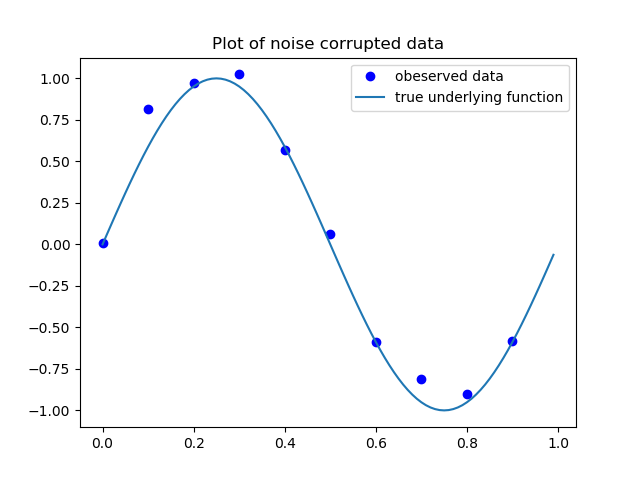
\includegraphics[width=\linewidth]{fig/figure_3.png}
  \caption{run time, accuracy performance comparsion ...}
  \label{fig:cf_vs_gd}
\end{figure}


Let us test some table here


\begin{table}[]
\centering
\begin{tabular}{|l|l|l|l|l|l|}
\hline
\textbf{Feature(s) w.r.t Performance}                                                                                                                                     & \textbf{\begin{tabular}[c]{@{}l@{}}MSE of \\ Training \\ Data\end{tabular}} & \textbf{\begin{tabular}[c]{@{}l@{}}MSE of \\ Validation \\ Data\end{tabular}} & \textbf{\begin{tabular}[c]{@{}l@{}}MSE of \\ Testing \\ Data\end{tabular}} & \textbf{\begin{tabular}[c]{@{}l@{}}run time \\ (in S)\end{tabular}} & \textbf{\begin{tabular}[c]{@{}l@{}}pre-run time \\ (in S) \\ time for \\ computing \\ text/numeric \\ features\\ and generate \\ related matrix\end{tabular}} \\ \hline
\textbf{\begin{tabular}[c]{@{}l@{}}Basic Model \\ (3 numeric  features)\end{tabular}}                                                                                     & 1.084683                                                                    & 1.020326                                                                      & 1.297531                                                                   & 0.027982                                                            & 3.207755                                                                                                                                                      \\ \hline
\textbf{Model With:}                                                                                                                                                      &                                                                             &                                                                               &                                                                            &                                                                     &                                                                                                                                                               \\ \hline
\textbf{“60 high frequency  words”}                                                                                                                                       & 1.059316                                                                    & 0.969286                                                                      & 1.298629                                                                   & 0.026985                                                            & 88.564367                                                                                                                                                     \\ \hline
                                                                                                                                                    \\ \hline
\end{tabular}
\caption{Performance Evaluation For Varies Implemented Features and Their Combinations}
\label{tbl:table_fp}
\end{table}


Provide results on the different models
you implemented (e.g., accuracy on the validation set, runtimes). You should report your leaderboard
test set accuracy in this section, but most of your results should be on your validation set (or from cross
validation).
\section{Discussion and Conclusion}(3+ Sentences)
\section{Division of Work}
\begin{itemize}
\item{\textbf{Robin Luo}}:
\item{\textbf{Marc-Andre Rousseau}}:
\item{\textbf{Bide Xu}}:
\end{itemize}
%\section{References}



\def\IEEEbibitemsep{0pt plus .5pt}
\bibliographystyle{IEEEtran}
%\bibliographystyle{IEEEtranS}
% argument is your BibTeX string definitions and bibliography database(s)
%\bibliography{IEEEabrv,../bib/paper}
\bibliography{bibfile}




\end{document}
%\begin{figure}[H]
%	\centering
%	\subfloat[MSE vs $\beta$ with 160 word feature vector]{{\includegraphics[width=5.5cm]{msevsbeta160} }}%
%	\qquad
%	\subfloat[MSE vs $\beta$ with 60 word feature vector]{{\includegraphics[width=5cm]{msevsbeta60words} }}
%	\caption{\textbf{A comparison the plots of MSE vs beta for 60 and 160 word feature vectors.}  The other hyperparameters were not constant and needed to be changed since what worked for 60 features did not work for 160.  Despite this, what we can see is a similar behaviour and shape between the two plots but with a difference in the scale.  The rise observed in plot B was also seen in other plots of A where the values were closer to zero than the ones seen in this diagram. }
%	\label{fig:betavsMSE}
%\end{figure} 